\chapter{実験}
2つの提案手法の評価と考察を行うために複数の実験を行った.

\section{HOPRDCにおける圧縮率と再圧縮率の関係} % (fold)
\label{sec:hoprdcにおける圧縮率と再圧縮率の関係}
\begin{figure}[tb]
\begin{center}
\includegraphics[clip, width=\columnwidth]{image/graph-recomp-comp.eps}
\caption{圧縮率と再圧縮率の関係}
\label{fig:image/graph-recomp-comp}
\end{center}
\end{figure}

% \begin{figure}[tb]
% \begin{center}
% 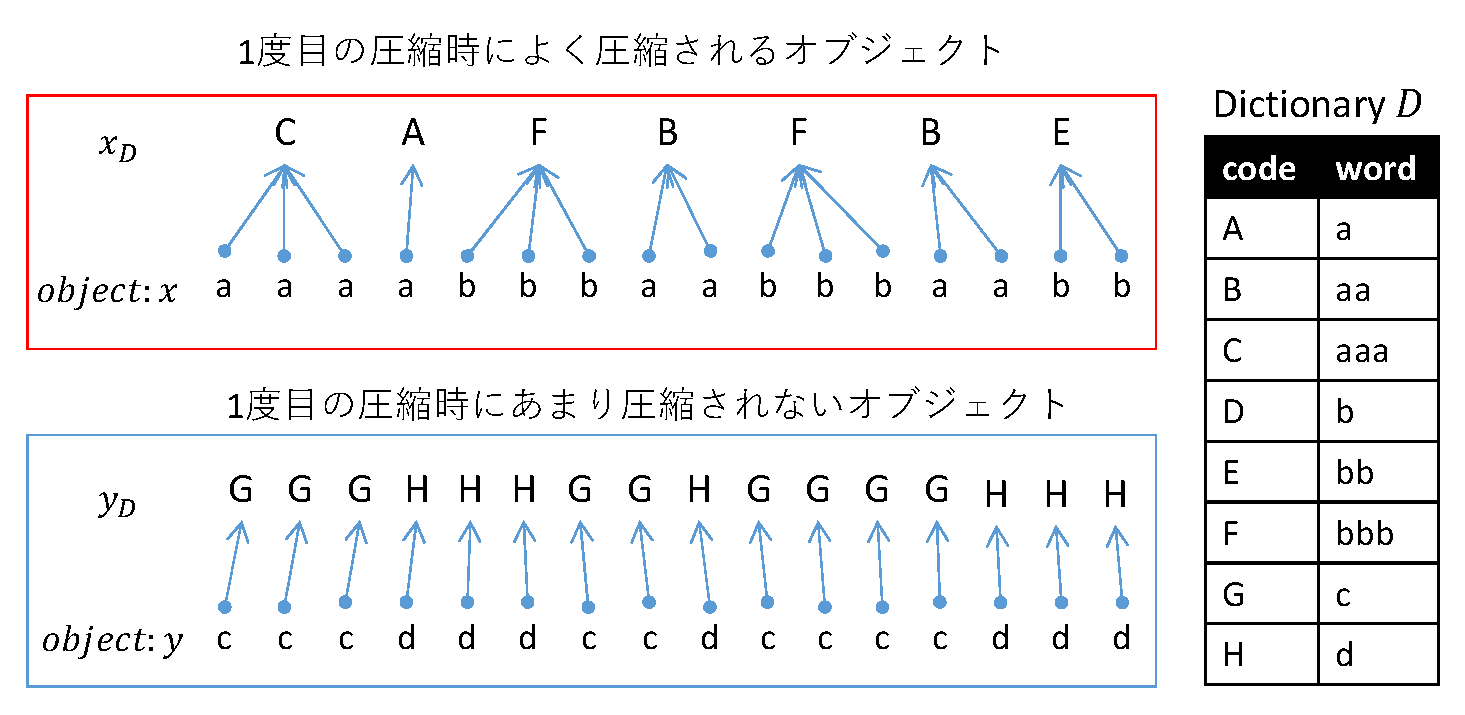
\includegraphics[clip, width=\columnwidth]{image/better-comp-object.eps}
% \caption{よく圧縮されるオブジェクトとあまり圧縮されないオブジェクト}
% \label{fig:image/better-comp-object.eps}
% \end{center}
% \end{figure}


圧縮率と再圧縮率の関係を調査する.
図~\ref{fig:image/graph-recomp-comp}は,Corelデータセットの画像を10個の辞書で圧縮したときの圧縮率と再圧縮率をプロットしたものである.画像ごとの違いを調べるために,11種類の画像をまとめてプロットした.
実験結果より,圧縮率と再圧縮率には負の相関がある,つまり1度目の圧縮でよく圧縮されたデータは,再圧縮時にはあまり圧縮できないことが分かった.
この理由は次のように考えられる.
\begin{itemize}
	\item $l $:入力オブジェクト長
	\item $l'$: $x$を$D$で圧縮したときの出力長
	\item $l''$: $x$を$D$で圧縮した符号列を,再圧縮したときの出力長
\end{itemize}
とするとき,圧縮率は$\frac{l'}{l}$,再圧縮率は$\frac{l''}{l'}$と表される.
ここで$\frac{l''}{l}$も(2回の圧縮を実行する)圧縮アルゴリズムで求めた圧縮率なので,$l''$は$l$が持つ情報量の近似とみなせる.そこで,$l''$を定数とすると,式\ref{eq:comp-recomp-relation}より圧縮率$\frac{l'}{l}$と再圧縮率$\frac{l''}{l'}$は反比例するので,負の相関関係が成り立つ.
\begin{equation}
\label{eq:comp-recomp-relation}
\frac{l'}{l}\times \frac{l''}{l'} = \frac{l''}{l} = 定数
\end{equation}


% 図\ref{fig:image/better-comp-object.eps}
% のように,辞書に登録されていない文字が連続して出現する場合,同じ符号が大量に出力される.その為,出力符号列は単純になり,2度目の圧縮時によく圧縮される.
% 画像ファイルでは,図\ref{fig:image/better-comp-object.eps}のように同じ文字が連続して出現しやすい.よって今回の実験で,圧縮率と再圧縮率に負の相関が見られたと考えられる.

% section hoprdcにおける圧縮率と再圧縮率の関係 (end)

\section{画像分類による性能評価}
\subsection{データセット}
以下の2種類のデータセットを用いて提案手法の画像分類性能を先行研究と比較した.
\begin{itemize}
	\item Corelデータセット~\cite{Corel}
	\item Caltech101 データセット~\cite{Caltech101}
\end{itemize}
\begin{figure}[tb]
\begin{center}
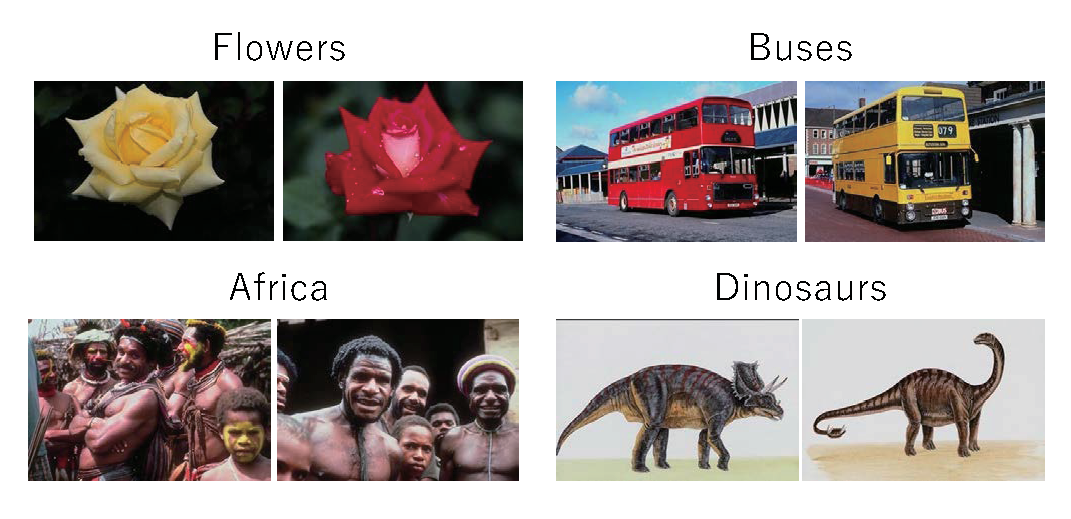
\includegraphics[clip, width=\columnwidth]{image/dataset.eps}
\caption{Corelデータセットの一部}
\label{fig:image/dataset.eps}
\end{center}
\end{figure}
Corelデータセットは先行研究~\cite{NMD}で実験に用いられたものと同じである.このデータセットはCorel image repository~\cite{Corel}の画像からなり,[256×384]か[384×256]の画像が1000枚,100枚づつ10個のクラスに分けられている.その一部を図\ref{fig:image/dataset.eps}に示す.
Caltech101データセットは画像分類においてよく用いられるデータセットである.このデータセットは9146枚の画像からなり,101個のカテゴリに分けられている.これらのカテゴリには少ないもので30枚,多いもので800枚の画像が含まれている.
\subsection{画像のテキスト化}
画像は2次元データなので,圧縮パターン認識に適用するには,1次元のテキストに変換する必要がある.
そこで,先行研究~\cite{NMD}と同様に,各画素のrgb値をそれぞれ5段階に量子化して,125種類の文字で表現し,これらを水平スキャンで連結してテキストに変換した.

\subsection{HOPRDCの評価結果}
PRDCとHOPRDCを比較するためCorelクラス分類実験を行う.
データセットからランダムに10枚画像を選択し,各画像から1つずつ,合計10個の基底辞書を作成する.その後ランダムに890枚選択した画像を学習画像とし,残りの画像100枚をクエリとして用いる.
クエリ画像の分類は次の手順で行う.
\begin{enumerate}
	\item クエリ画像を圧縮率ベクトルに変換する
	\item クエリ画像をk-NN法でクラス分類する.クエリと最近の$k$枚の学習画像を求め,その中で枚数が最も多いクラスに分類する.
\end{enumerate}
今回の実験では$k$=5とした.
判別率$r$は次のように計算する.
\begin{equation}
r=\frac{正しく分類されたテスト画像数}{テスト画像数}
\end{equation}

% 各クラス$c$の判別率$r_c$は次のように計算する.
% \begin{equation}
% r_c=\frac{正しく分類されたクラスcのデータ数}{テスト画像中のクラスcのデータ数}
% \end{equation}

\begin{figure}[tb]
\begin{center}
\includegraphics[clip, width=\columnwidth]{image/PRDCvsProposed.eps}
\caption{クラス毎の判別率(クエリの数は100枚,基底辞書の個数は10個,試行回数は300回)}
\label{fig:PRDCvsProposed.eps}
\end{center}
\end{figure}
\begin{table}
\caption{全画像に対する判別率}
\label{tab:Average_PRDCvsProposed}
\begin{center}
\begin{tabular}{|l||l|}
\hline
PRDC   & 0.6393 \\
\hline
HOPRDC & 0.6798 \\
\hline
\end{tabular}
\end{center}
\end{table}
本実験では基底辞書をランダムに選択するため,300回の試行を行いその平均値を報告する.

表\ref{tab:Average_PRDCvsProposed}は前テスト画像に対する判別率である.HOPRDCはPRDCに比べて4\%程度判別率が向上した.
図\ref{fig:PRDCvsProposed.eps}はクラスごとの判別率である.
提案手法では,BusクラスやFlowerクラスにおいてPRDCを大きく上回った.この2つのクラスのインスタンスには,同じ形で色が違うものが含まれる.PRDCでは,単語の頻度のみを考慮しているため,オブジェクトの色に認識結果が大きく左右される.一方,提案手法では,再圧縮率により単語の隣接関係を考慮するため,オブジェクトの形も認識結果に影響を与える.

図\ref{fig:PRDC_HOPRDC_retrival.eps}はPRDCとHOPRDCで作成したベクトルを用いて,類似画像検索を行った結果の一例である.PRDCでは,赤い色のピクセルの割合がクエリ画像と似ているものが上位に来ている.HOPRDCでは,赤いピクセルの割合が似ているだけではなく,赤いピクセルの形が似ているものが上位に来ている.
再圧縮率で単語の順序関係を考慮したことで,オブジェクトの形が似ているものが抽出されやすくなったことが確認できる.

\begin{figure}[tb]
\centering
\includegraphics[clip, width=\columnwidth]{image/PRDC_HOPRDC_retrival.eps}
\caption{PRDCとHOPRDCの類似画像検索結果例}
\label{fig:PRDC_HOPRDC_retrival.eps}
\end{figure}


\subsection{WNMDの評価結果}
提案手法であるWNMDと,現在辞書間距離の中で最も精度が高いNMDを比較するため,2つのデータセットを使い類似画像検索を行う.
Corelデータセットを用いた実験では,データベースに1000枚の画像全てを登録する.クエリはこの中の1枚を使用する.クエリとデータベースの全画像間で類似度計算を行い,類似度が高い上位100枚の画像を検索結果とする.
クエリ画像$Q$に対する検索結果は式(\ref{equ:Precision_Corel})に示す適合率で評価する.分母の100は検索結果の画像数であるが,1クラスあたりの画像数とも一致する.
\begin{equation}
P(Q) = \frac{N_r}{100}
\label{equ:Precision_Corel}
\end{equation}
ここで$N_r$は検索結果の中でクエリ画像Qと同じクラスの画像の枚数である.
全ての画像をクエリとして使い,1000回類似画像検索を行った平均適合率によりアルゴリズムの性能を評価する.

Caltech101データセットを用いた実験では,データベースに9146枚の画像全てを登録する.クエリはこの中の1枚を使用する.クエリとデータベースの全画像間で類似度計算を行い,類似度が高い上位30枚の画像を検索結果とする.
クエリ画像$Q$に対する検索結果は式(\ref{equ:Precision_Caltech})に示す適合率で評価する.分母の30は検索結果の画像数である.
\begin{equation}
P(Q) = \frac{N_r}{30}
\label{equ:Precision_Caltech}
\end{equation}

\begin{figure}[tb]
\begin{center}
\includegraphics[clip, width=\columnwidth]{image/NMDvsProposed.eps}
\caption{NMDと提案手法の平均適合率の比較(クエリはデータセット中の全ての画像)}
\label{fig:NMDvsProposed.eps}
\end{center}
\end{figure}
\begin{table}
\caption{全画像に対する平均適合率}
\label{tab:Average_NMDvsProposed}
\begin{center}
\begin{tabular}{|l||l|l|}
\hline
&Corel&Caltech101 \\
\hline
NMD  & 0.509 & 0.312\\
\hline
WNMD & 0.530 & 0.337\\
\hline
\end{tabular}
\end{center}
\end{table}

% Table generated by Excel2LaTeX from sheet 'Sheet1'
\begin{table}[htbp]
\centering
\caption{重みの評価}
\begin{tabular}{|l|r|}
\hline
\textbf{重み} &
\multicolumn{1}{l|}{\textbf{適合率}}
\bigstrut\\
\hline
$\log_2 (|w|+1)$ &
0.524
\bigstrut\\
\hline
$\sqrt{|w|}$ &
0.53
\bigstrut\\
\hline
$|w|$ &
0.519
\bigstrut\\
\hline
    \end{tabular}%
  \label{tab:NMD_weight_compare}%
\end{table}%

表\ref{tab:Average_NMDvsProposed}に全画像に対する平均適合率を示す.
CorelデータセットではWNMDはNMDと比べて1.6\%程度適合率が向上した.
Caltech101データセットでは約2.5\%適合率が向上した.

WNMDがどのような画像に対して有効に働いているかを知るために,Corelデータセットに対しての結果を詳しく調べる.
図\ref{fig:NMDvsProposed.eps}にNMDとWNMDのクラスごとの平均適合率を示す.
提案手法ではAfricaクラスや,DinosaursクラスにおいてNMDを大きく上回った.
この2つのクラスでは,同色で単純な領域が広い面積を占める画像が多い.
Africaクラスには人物を映した画像が多く,肌色の単純な領域が大きい.
Dinosoursクラスでは,背景や恐竜の肌が少ない色で表現されており,単純である.
NMDでは単純領域の特徴を軽視するのに対し,WNMDでは,単語に長さに応じた重みをつけることで,これらのクラスで重要な特徴となる単純な領域を軽視せずに類似計算を行うことができ,精度が向上した.
\subsection{重み付け関数$g(w)$の評価} % (fold)
\label{sub:重み付け関数}
長さに対する重みが適切かどうかの実験を行った.
単語$w$の長さを$|w|$としたとき,$\sqrt{|w|}$,$|w|$,$\log_2 (|w|+1)$の3種類の重みを比較した.
ここで,$log_2(|w|+1)$は,全ての文字が同じ単語の情報量,$|w|$は全ての文字が違う単語の情報量である.
比較はCorelデータセットで式\ref{equ:Precision_Corel}を用いて行った.結果は表~\ref{tab:NMD_weight_compare}に示す.実験より,$\sqrt{|w|}$が最も高い精度であることがわかる.

% subsection 重み付け関数 (end)

\section{時系列データ分類による性能評価} % (fold)
\label{sub:時系列データ分類による性能評価}
提案手法が画像以外のデータセットに対して有効かどうかを調べるために,様々な種類の時系列データに対して分類実験を行った.
\subsection{UCR Time Series Classification Archive} % (fold)
\label{sub:UCR Time Series Classification Archive}
UCR Time Series Classification Archive~\cite{UCRArchive}(以下 UCR Archive)は,様々な種類の時系列データを集めたデータセット集である.
現在このデータセット集には全部で85種類のデータセットが用意されており,全てが同じフォーマットで記述されている.そのため,手軽に多種多様なデータに対しての分類精度を比較することができる.
% subsection UCR Time Series Classification Archive (end)
\subsection{データのテキスト化} % (fold)
\label{sub:データのテキスト化}
圧縮パターン認識に適用するために,時系列データを1次元のテキストに変換する.
全てのTESTデータとTRAINデータの値を125,60,30,15レベルに量子化し,文字に置き換えた.

\begin{figure}[tb]
\begin{center}
\includegraphics[clip, width=\columnwidth]{image/DataEncode.eps}
\end{center}
\caption{データのテキスト化}
\label{fig:DataEncode.eps}
\end{figure}
% subsection subsection_name (end)

\subsection{クラス分類実験} % (fold)
\label{sub:クラス分類実験}
クラス分類実験の方法について説明する.
UCRArchiveのデータセットはそれぞれTESTデータとTRAINデータに予め分けられている.
実験では,TRAINデータを用いて,TESTデータを1-NNでクラス分類したときの分類精度を評価する.

PRDC・HOPRDCを用いた分類実験では,TRAINデータの各クラスから2つずつデータを選び,それを基底辞書として用いる.(例えば,3クラス分類の場合,基底辞書は全部で6つ,PRDCでは6次元,HOPRDCでは12次元のベクトルが作成される.)
TESTデータから作成した圧縮率ベクトルとTRAINデータの圧縮率ベクトルとのユークリッド距離を用いて1-NN分類を行う.
このとき,基底辞書の選択により分類精度が変動するので,100回の分類実験を行いその平均を評価する.

NMD・WNMDを用いた分類実験では,TESTデータとTRAINデータから辞書を作成し,辞書間距離NMD・WNMDを用いて1-NN分類を行う.
% subsection クラス分類実験 (end)
\subsection{実験結果} % (fold)
\label{sub:実験結果}
表\ref{tab:HOPRDC_UP_AND_DOWN},表\ref{tab:WNMD_UP_AND_DOWN}に実験の結果,精度が向上したデータセットの個数と,変化しなかった個数,低下した個数をまとめた.結果の詳細は付録に掲載する.
実験より,HOPRDC,WNMDは多くのデータセットに対し,有効であるという結果が得られた.しかし,精度が低下してしまったデータセットも存在するので,どのようなデータについて有効なのかを詳しく考察する.

HOPRDCでは図\ref{fig:image/HOPRDC_up_down.eps}左のようなデータセットでは精度が低下した.このデータセットは全てのデータの大まかな構造が同じなので,クラス分類においては細かい部分の違いが大きく影響する.HOPRDCではデータの大まかな構造を重視するため,精度が低下したと考えられる.このようなデータセットは,データの記述に数値の微分を用いると,データの特徴を表現でき,うまく分類できるようになると考えられる.
逆に,図\ref{fig:image/HOPRDC_up_down.eps}右のような,カテゴリごとにデータの大まかな形が異なるデータセットでは,大きく精度が向上した.また,データを15分割したとき,HOPRDCは先行研究と比べて大きな向上が見られなかった.15分割では多くのデータが同じような形で表現されるので,HOPRDCで用いている単語の隣接関係の情報があまり役に立たないことが原因と考えられる.

WNMDでは,図~\ref{fig:image/WNMD_up_down.eps}左側のような,数値の高さのみが分類に重要なデータセットでは精度が低下した.逆に,分類にデータの数値が出現する位置が重要なデータで精度が向上した.
また,125分割,60分割のとき,WNMDは先行研究と比べ同程度の結果となったが,これはデータから作成された辞書中に長い単語が殆ど出現していないことが要因である.

% Table generated by Excel2LaTeX from sheet 'Sheet1'
\begin{table}[htbp]
\centering
\caption{HOPRDCでPRDCよりも精度が向上(低下)したデータセットの数}
\begin{tabular}{|l|r|r|r|r|}
\cline{2-5}    \multicolumn{1}{r|}{} &
\multicolumn{1}{c|}{125分割} &
\multicolumn{1}{c|}{60分割} &
\multicolumn{1}{c|}{30分割} &
\multicolumn{1}{c|}{15分割}
\bigstrut\\
\hline
向上 &
52 &
51 &
51 &
40
\bigstrut\\
\hline
変化なし &
0 &
2 &
2 &
2
\bigstrut\\
\hline
低下 &
26 &
25 &
25 &
36
\bigstrut\\
\hline
    \end{tabular}%
  \label{tab:HOPRDC_UP_AND_DOWN}%
\end{table}%

% Table generated by Excel2LaTeX from sheet 'Sheet1'
\begin{table}[htbp]
\centering
\caption{WNMDでNMDよりも精度が向上(低下)したデータセットの数}
\begin{tabular}{|l|r|r|r|r|}
\cline{2-5}    \multicolumn{1}{r|}{} &
\multicolumn{1}{c|}{125分割} &
\multicolumn{1}{c|}{60分割} &
\multicolumn{1}{c|}{30分割} &
\multicolumn{1}{c|}{15分割}
\bigstrut\\
\hline
向上 &
41 &
41 &
49 &
47
\bigstrut\\
\hline
変化なし &
9 &
4 &
5 &
7
\bigstrut\\
\hline
低下 &
35 &
40 &
31 &
31
\bigstrut\\
\hline
    \end{tabular}%
  \label{tab:WNMD_UP_AND_DOWN}%
\end{table}%


% subsection 実験結果 (end)
% % Table generated by Excel2LaTeX from sheet 'split30 k=1'
\begin{longtable}[c]{|l||r||r|r||r|r|}
\caption{データを30分割したときの精度比較}
\\
\hline
\textbf{データセット名} &
\multicolumn{1}{l||}{\textbf{Euclidean}} &
\multicolumn{1}{l|}{\textbf{PRDC}} &
\multicolumn{1}{l||}{\textbf{HOPRDC}} &
\multicolumn{1}{l|}{\textbf{NMD}} &
\multicolumn{1}{l|}{\textbf{WNMD}}
\bigstrut\\
\hline
\endhead
\rowcolor[rgb]{ .851,  .851,  .851} 50words &
0.631 &
&
&
0.321 &
\cellcolor[rgb]{ .973,  .796,  .678} \textbf{0.327}
\bigstrut[t]\\
Adiac &
0.611 &
\cellcolor[rgb]{ .973,  .796,  .678} \textbf{0.459} &
0.39 &
0.317 &
\cellcolor[rgb]{ .973,  .796,  .678} \textbf{0.345}
\\
\rowcolor[rgb]{ .851,  .851,  .851} ArrowHead &
0.8 &
\cellcolor[rgb]{ .973,  .796,  .678} \textbf{0.597} &
0.582 &
\cellcolor[rgb]{ .973,  .796,  .678} \textbf{0.651} &
0.629
\\
Beef &
0.667 &
\cellcolor[rgb]{ .973,  .796,  .678} \textbf{0.45} &
0.443 &
0.567 &
\cellcolor[rgb]{ .973,  .796,  .678} \textbf{0.6}
\\
\rowcolor[rgb]{ .851,  .851,  .851} BeetleFly &
0.75 &
\cellcolor[rgb]{ .973,  .796,  .678} \textbf{0.735} &
0.66 &
0.8 &
\cellcolor[rgb]{ .973,  .796,  .678} \textbf{0.9}
\\
BirdChicken &
0.55 &
0.745 &
\cellcolor[rgb]{ .973,  .796,  .678} \textbf{0.765} &
0.8 &
\cellcolor[rgb]{ .973,  .796,  .678} \textbf{0.85}
\\
\rowcolor[rgb]{ .851,  .851,  .851} Car &
0.733 &
0.41 &
\cellcolor[rgb]{ .973,  .796,  .678} \textbf{0.43} &
0.583 &
\cellcolor[rgb]{ .973,  .796,  .678} \textbf{0.667}
\\
CBF &
0.852 &
\cellcolor[rgb]{ .973,  .796,  .678} \textbf{0.641} &
0.639 &
\cellcolor[rgb]{ .973,  .796,  .678} \textbf{0.661} &
0.659
\\
\rowcolor[rgb]{ .851,  .851,  .851} ChlorineConcentration &
0.65 &
0.499 &
\cellcolor[rgb]{ .973,  .796,  .678} \textbf{0.504} &
\cellcolor[rgb]{ .973,  .796,  .678} \textbf{0.547} &
0.541
\\
CinC\_ECG\_torso &
0.897 &
0.446 &
\cellcolor[rgb]{ .973,  .796,  .678} \textbf{0.544} &
\cellcolor[rgb]{ .973,  .796,  .678} \textbf{0.605} &
0.594
\\
\rowcolor[rgb]{ .851,  .851,  .851} Coffee &
1 &
0.618 &
\cellcolor[rgb]{ .973,  .796,  .678} \textbf{0.629} &
\cellcolor[rgb]{ .973,  .796,  .678} \textbf{0.821} &
0.786
\\
Computers &
0.576 &
0.62 &
\cellcolor[rgb]{ .973,  .796,  .678} \textbf{0.629} &
\cellcolor[rgb]{ .973,  .796,  .678} \textbf{0.612} &
0.58
\\
\rowcolor[rgb]{ .851,  .851,  .851} Cricket\_X &
0.577 &
\cellcolor[rgb]{ .973,  .796,  .678} \textbf{0.409} &
0.403 &
0.426 &
\cellcolor[rgb]{ .973,  .796,  .678} \textbf{0.436}
\\
Cricket\_Y &
0.567 &
\cellcolor[rgb]{ .973,  .796,  .678} \textbf{0.359} &
0.353 &
0.405 &
\cellcolor[rgb]{ .973,  .796,  .678} \textbf{0.436}
\\
\rowcolor[rgb]{ .851,  .851,  .851} Cricket\_Z &
0.587 &
\cellcolor[rgb]{ .973,  .796,  .678} \textbf{0.375} &
0.373 &
0.41 &
\cellcolor[rgb]{ .973,  .796,  .678} \textbf{0.413}
\\
DiatomSizeReduction &
0.935 &
&
&
0.846 &
\cellcolor[rgb]{ .973,  .796,  .678} \textbf{0.859}
\\
\rowcolor[rgb]{ .851,  .851,  .851} DistalPhalanxOutlineAgeGroup &
0.783 &
0.727 &
\cellcolor[rgb]{ .973,  .796,  .678} \textbf{0.75} &
\cellcolor[rgb]{ .973,  .796,  .678} \textbf{0.728} &
0.723
\\
DistalPhalanxOutlineCorrect &
0.752 &
0.661 &
\cellcolor[rgb]{ .973,  .796,  .678} \textbf{0.664} &
0.695 &
\cellcolor[rgb]{ .973,  .796,  .678} \textbf{0.698}
\\
\rowcolor[rgb]{ .851,  .851,  .851} DistalPhalanxTW &
0.728 &
0.691 &
\cellcolor[rgb]{ .973,  .796,  .678} \textbf{0.692} &
0.688 &
\cellcolor[rgb]{ .973,  .796,  .678} \textbf{0.698}
\\
Earthquakes &
0.674 &
0.73 &
\cellcolor[rgb]{ .973,  .796,  .678} \textbf{0.731} &
0.724 &
\cellcolor[rgb]{ .973,  .796,  .678} \textbf{0.733}
\\
\rowcolor[rgb]{ .851,  .851,  .851} ECG200 &
0.88 &
0.6 &
\cellcolor[rgb]{ .973,  .796,  .678} \textbf{0.652} &
\cellcolor[rgb]{ .973,  .796,  .678} \textbf{0.7} &
0.69
\\
ECG5000 &
0.925 &
&
&
0.899 &
\cellcolor[rgb]{ .973,  .796,  .678} \textbf{0.902}
\\
\rowcolor[rgb]{ .851,  .851,  .851} ECGFiveDays &
0.797 &
0.632 &
\cellcolor[rgb]{ .973,  .796,  .678} \textbf{0.674} &
0.741 &
\cellcolor[rgb]{ .973,  .796,  .678} \textbf{0.746}
\\
ElectricDevices &
0.549 &
0.561 &
\cellcolor[rgb]{ .973,  .796,  .678} \textbf{0.607} &
0.631 &
\cellcolor[rgb]{ .973,  .796,  .678} \textbf{0.633}
\\
\rowcolor[rgb]{ .851,  .851,  .851} FaceAll &
0.714 &
\cellcolor[rgb]{ .973,  .796,  .678} \textbf{0.296} &
0.294 &
0.325 &
\cellcolor[rgb]{ .973,  .796,  .678} \textbf{0.37}
\\
FaceFour &
0.784 &
0.51 &
\cellcolor[rgb]{ .973,  .796,  .678} \textbf{0.52} &
\cellcolor[rgb]{ .973,  .796,  .678} \textbf{0.636} &
0.625
\\
\rowcolor[rgb]{ .851,  .851,  .851} FacesUCR &
0.769 &
\cellcolor[rgb]{ .973,  .796,  .678} \textbf{0.382} &
0.374 &
0.411 &
\cellcolor[rgb]{ .973,  .796,  .678} \textbf{0.428}
\\
FISH &
0.783 &
0.237 &
0.237 &
\cellcolor[rgb]{ .973,  .796,  .678} \textbf{0.44} &
0.429
\\
\rowcolor[rgb]{ .851,  .851,  .851} FordA &
0.659 &
0.629 &
\cellcolor[rgb]{ .973,  .796,  .678} \textbf{0.653} &
0.61 &
\cellcolor[rgb]{ .973,  .796,  .678} \textbf{0.618}
\\
FordB &
0.558 &
0.615 &
\cellcolor[rgb]{ .973,  .796,  .678} \textbf{0.635} &
0.534 &
\cellcolor[rgb]{ .973,  .796,  .678} \textbf{0.561}
\\
\rowcolor[rgb]{ .851,  .851,  .851} Gun\_Point &
0.913 &
0.788 &
\cellcolor[rgb]{ .973,  .796,  .678} \textbf{0.793} &
\cellcolor[rgb]{ .973,  .796,  .678} \textbf{0.867} &
0.86
\\
Ham &
0.6 &
0.481 &
\cellcolor[rgb]{ .973,  .796,  .678} \textbf{0.485} &
0.457 &
\cellcolor[rgb]{ .973,  .796,  .678} \textbf{0.524}
\\
\rowcolor[rgb]{ .851,  .851,  .851} HandOutlines &
0.801 &
\cellcolor[rgb]{ .973,  .796,  .678} \textbf{0.645} &
0.628 &
0.666 &
\cellcolor[rgb]{ .973,  .796,  .678} \textbf{0.682}
\\
Haptics &
0.37 &
0.238 &
\cellcolor[rgb]{ .973,  .796,  .678} \textbf{0.255} &
\cellcolor[rgb]{ .973,  .796,  .678} \textbf{0.266} &
0.227
\\
\rowcolor[rgb]{ .851,  .851,  .851} Herring &
0.516 &
\cellcolor[rgb]{ .973,  .796,  .678} \textbf{0.563} &
0.497 &
0.594 &
0.594
\\
InlineSkate &
0.342 &
\cellcolor[rgb]{ .973,  .796,  .678} \textbf{0.277} &
0.259 &
0.351 &
\cellcolor[rgb]{ .973,  .796,  .678} \textbf{0.356}
\\
\rowcolor[rgb]{ .851,  .851,  .851} InsectWingbeatSound &
0.562 &
0.159 &
\cellcolor[rgb]{ .973,  .796,  .678} \textbf{0.169} &
0.178 &
\cellcolor[rgb]{ .973,  .796,  .678} \textbf{0.183}
\\
ItalyPowerDemand &
0.955 &
\cellcolor[rgb]{ .973,  .796,  .678} \textbf{0.615} &
0.613 &
0.729 &
\cellcolor[rgb]{ .973,  .796,  .678} \textbf{0.736}
\\
\rowcolor[rgb]{ .851,  .851,  .851} LargeKitchenAppliances &
0.493 &
\cellcolor[rgb]{ .973,  .796,  .678} \textbf{0.661} &
0.6 &
\cellcolor[rgb]{ .973,  .796,  .678} \textbf{0.739} &
0.699
\\
Lighting2 &
0.754 &
\cellcolor[rgb]{ .973,  .796,  .678} \textbf{0.693} &
0.69 &
0.656 &
0.656
\\
\rowcolor[rgb]{ .851,  .851,  .851} Lighting7 &
0.575 &
0.484 &
\cellcolor[rgb]{ .973,  .796,  .678} \textbf{0.512} &
0.589 &
\cellcolor[rgb]{ .973,  .796,  .678} \textbf{0.616}
\\
MALLAT &
0.914 &
&
&
0.831 &
\cellcolor[rgb]{ .973,  .796,  .678} \textbf{0.839}
\\
\rowcolor[rgb]{ .851,  .851,  .851} Meat &
0.933 &
0.557 &
\cellcolor[rgb]{ .973,  .796,  .678} \textbf{0.6} &
0.883 &
0.883
\\
MedicalImages &
0.684 &
0.485 &
\cellcolor[rgb]{ .973,  .796,  .678} \textbf{0.494} &
\cellcolor[rgb]{ .973,  .796,  .678} \textbf{0.568} &
0.551
\\
\rowcolor[rgb]{ .851,  .851,  .851} MiddlePhalanxOutlineAgeGroup &
0.74 &
0.72 &
\cellcolor[rgb]{ .973,  .796,  .678} \textbf{0.722} &
\cellcolor[rgb]{ .973,  .796,  .678} \textbf{0.735} &
0.715
\\
MiddlePhalanxOutlineCorrect &
0.753 &
0.53 &
0.53 &
0.603 &
\cellcolor[rgb]{ .973,  .796,  .678} \textbf{0.61}
\\
\rowcolor[rgb]{ .851,  .851,  .851} MiddlePhalanxTW &
0.561 &
0.551 &
\cellcolor[rgb]{ .973,  .796,  .678} \textbf{0.559} &
\cellcolor[rgb]{ .973,  .796,  .678} \textbf{0.579} &
0.574
\\
MoteStrain &
0.879 &
0.653 &
\cellcolor[rgb]{ .973,  .796,  .678} \textbf{0.671} &
\cellcolor[rgb]{ .973,  .796,  .678} \textbf{0.74} &
0.736
\\
\rowcolor[rgb]{ .851,  .851,  .851} NonInvasiveFatalECG\_Thorax1 &
0.829 &
\cellcolor[rgb]{ .973,  .796,  .678} \textbf{0.518} &
0.465 &
0.518 &
0.518
\\
NonInvasiveFatalECG\_Thorax2 &
0.88 &
\cellcolor[rgb]{ .973,  .796,  .678} \textbf{0.567} &
0.533 &
\cellcolor[rgb]{ .973,  .796,  .678} \textbf{0.619} &
0.608
\\
\rowcolor[rgb]{ .851,  .851,  .851} OliveOil &
0.867 &
0.567 &
\cellcolor[rgb]{ .973,  .796,  .678} \textbf{0.583} &
\cellcolor[rgb]{ .973,  .796,  .678} \textbf{0.833} &
0.8
\\
OSULeaf &
0.521 &
0.464 &
\cellcolor[rgb]{ .973,  .796,  .678} \textbf{0.465} &
0.537 &
\cellcolor[rgb]{ .973,  .796,  .678} \textbf{0.541}
\\
\rowcolor[rgb]{ .851,  .851,  .851} PhalangesOutlinesCorrect &
0.761 &
\cellcolor[rgb]{ .973,  .796,  .678} \textbf{0.605} &
0.6 &
0.652 &
\cellcolor[rgb]{ .973,  .796,  .678} \textbf{0.662}
\\
Phoneme &
0.109 &
&
&
0.197 &
\cellcolor[rgb]{ .973,  .796,  .678} \textbf{0.206}
\\
\rowcolor[rgb]{ .851,  .851,  .851} Plane &
0.962 &
\cellcolor[rgb]{ .973,  .796,  .678} \textbf{0.901} &
0.889 &
0.962 &
0.962
\\
ProximalPhalanxOutlineAgeGroup &
0.785 &
\cellcolor[rgb]{ .973,  .796,  .678} \textbf{0.747} &
0.735 &
\cellcolor[rgb]{ .973,  .796,  .678} \textbf{0.829} &
0.805
\\
\rowcolor[rgb]{ .851,  .851,  .851} ProximalPhalanxOutlineCorrect &
0.808 &
0.675 &
\cellcolor[rgb]{ .973,  .796,  .678} \textbf{0.676} &
0.715 &
\cellcolor[rgb]{ .973,  .796,  .678} \textbf{0.725}
\\
ProximalPhalanxTW &
0.708 &
&
&
0.678 &
\cellcolor[rgb]{ .973,  .796,  .678} \textbf{0.693}
\\
\rowcolor[rgb]{ .851,  .851,  .851} RefrigerationDevices &
0.395 &
0.445 &
\cellcolor[rgb]{ .973,  .796,  .678} \textbf{0.476} &
\cellcolor[rgb]{ .973,  .796,  .678} \textbf{0.485} &
0.475
\\
ScreenType &
0.36 &
0.379 &
\cellcolor[rgb]{ .973,  .796,  .678} \textbf{0.405} &
0.424 &
\cellcolor[rgb]{ .973,  .796,  .678} \textbf{0.443}
\\
\rowcolor[rgb]{ .851,  .851,  .851} ShapeletSim &
0.539 &
0.513 &
\cellcolor[rgb]{ .973,  .796,  .678} \textbf{0.532} &
0.594 &
\cellcolor[rgb]{ .973,  .796,  .678} \textbf{0.628}
\\
ShapesAll &
0.752 &
\cellcolor[rgb]{ .973,  .796,  .678} \textbf{0.606} &
0.597 &
0.617 &
\cellcolor[rgb]{ .973,  .796,  .678} \textbf{0.647}
\\
\rowcolor[rgb]{ .851,  .851,  .851} SmallKitchenAppliances &
0.344 &
0.505 &
\cellcolor[rgb]{ .973,  .796,  .678} \textbf{0.568} &
0.533 &
\cellcolor[rgb]{ .973,  .796,  .678} \textbf{0.539}
\\
SonyAIBORobotSurface &
0.696 &
\cellcolor[rgb]{ .973,  .796,  .678} \textbf{0.638} &
0.599 &
\cellcolor[rgb]{ .973,  .796,  .678} \textbf{0.632} &
0.631
\\
\rowcolor[rgb]{ .851,  .851,  .851} SonyAIBORobotSurfaceII &
0.859 &
\cellcolor[rgb]{ .973,  .796,  .678} \textbf{0.571} &
0.57 &
0.633 &
\cellcolor[rgb]{ .973,  .796,  .678} \textbf{0.636}
\\
StarLightCurves &
0.849 &
0.858 &
\cellcolor[rgb]{ .973,  .796,  .678} \textbf{0.881} &
0.84 &
\cellcolor[rgb]{ .973,  .796,  .678} \textbf{0.848}
\\
\rowcolor[rgb]{ .851,  .851,  .851} Strawberry &
0.938 &
0.692 &
\cellcolor[rgb]{ .973,  .796,  .678} \textbf{0.714} &
0.889 &
\cellcolor[rgb]{ .973,  .796,  .678} \textbf{0.891}
\\
SwedishLeaf &
0.789 &
\cellcolor[rgb]{ .973,  .796,  .678} \textbf{0.651} &
0.643 &
0.598 &
\cellcolor[rgb]{ .973,  .796,  .678} \textbf{0.614}
\\
\rowcolor[rgb]{ .851,  .851,  .851} Symbols &
0.899 &
0.569 &
\cellcolor[rgb]{ .973,  .796,  .678} \textbf{0.659} &
\cellcolor[rgb]{ .973,  .796,  .678} \textbf{0.758} &
0.75
\\
synthetic\_control &
0.88 &
0.308 &
\cellcolor[rgb]{ .973,  .796,  .678} \textbf{0.317} &
0.307 &
\cellcolor[rgb]{ .973,  .796,  .678} \textbf{0.317}
\\
\rowcolor[rgb]{ .851,  .851,  .851} ToeSegmentation1 &
0.68 &
0.641 &
\cellcolor[rgb]{ .973,  .796,  .678} \textbf{0.661} &
0.724 &
\cellcolor[rgb]{ .973,  .796,  .678} \textbf{0.732}
\\
ToeSegmentation2 &
0.808 &
0.698 &
\cellcolor[rgb]{ .973,  .796,  .678} \textbf{0.712} &
0.862 &
\cellcolor[rgb]{ .973,  .796,  .678} \textbf{0.877}
\\
\rowcolor[rgb]{ .851,  .851,  .851} Trace &
0.76 &
0.823 &
\cellcolor[rgb]{ .973,  .796,  .678} \textbf{0.891} &
0.88 &
\cellcolor[rgb]{ .973,  .796,  .678} \textbf{0.9}
\\
Two\_Patterns &
0.907 &
0.266 &
\cellcolor[rgb]{ .973,  .796,  .678} \textbf{0.275} &
0.346 &
\cellcolor[rgb]{ .973,  .796,  .678} \textbf{0.393}
\\
\rowcolor[rgb]{ .851,  .851,  .851} TwoLeadECG &
0.747 &
0.686 &
\cellcolor[rgb]{ .973,  .796,  .678} \textbf{0.761} &
\cellcolor[rgb]{ .973,  .796,  .678} \textbf{0.862} &
0.844
\\
uWaveGestureLibrary\_X &
0.739 &
0.352 &
\cellcolor[rgb]{ .973,  .796,  .678} \textbf{0.37} &
\cellcolor[rgb]{ .973,  .796,  .678} \textbf{0.411} &
0.408
\\
\rowcolor[rgb]{ .851,  .851,  .851} uWaveGestureLibrary\_Y &
0.662 &
0.304 &
\cellcolor[rgb]{ .973,  .796,  .678} \textbf{0.325} &
\cellcolor[rgb]{ .973,  .796,  .678} \textbf{0.365} &
0.364
\\
uWaveGestureLibrary\_Z &
0.65 &
0.37 &
\cellcolor[rgb]{ .973,  .796,  .678} \textbf{0.39} &
\cellcolor[rgb]{ .973,  .796,  .678} \textbf{0.456} &
0.453
\\
\rowcolor[rgb]{ .851,  .851,  .851} UWaveGestureLibraryAll &
0.948 &
0.279 &
\cellcolor[rgb]{ .973,  .796,  .678} \textbf{0.332} &
0.384 &
\cellcolor[rgb]{ .973,  .796,  .678} \textbf{0.387}
\\
wafer &
0.995 &
0.95 &
\cellcolor[rgb]{ .973,  .796,  .678} \textbf{0.958} &
0.977 &
\cellcolor[rgb]{ .973,  .796,  .678} \textbf{0.978}
\\
\rowcolor[rgb]{ .851,  .851,  .851} Wine &
0.611 &
0.469 &
\cellcolor[rgb]{ .973,  .796,  .678} \textbf{0.5} &
\cellcolor[rgb]{ .973,  .796,  .678} \textbf{0.481} &
0.444
\\
WordsSynonyms &
0.618 &
&
&
\cellcolor[rgb]{ .973,  .796,  .678} \textbf{0.331} &
0.317
\\
\rowcolor[rgb]{ .851,  .851,  .851} Worms &
0.365 &
0.397 &
\cellcolor[rgb]{ .973,  .796,  .678} \textbf{0.447} &
\cellcolor[rgb]{ .973,  .796,  .678} \textbf{0.552} &
0.541
\\
WormsTwoClass &
0.586 &
0.583 &
\cellcolor[rgb]{ .973,  .796,  .678} \textbf{0.604} &
\cellcolor[rgb]{ .973,  .796,  .678} \textbf{0.674} &
0.657
\\
\rowcolor[rgb]{ .851,  .851,  .851} yoga &
0.83 &
0.578 &
\cellcolor[rgb]{ .973,  .796,  .678} \textbf{0.58} &
0.731 &
\cellcolor[rgb]{ .973,  .796,  .678} \textbf{0.743}
\bigstrut[b]\\
\hline
\end{longtable}%


% \LTXtable{\columnwidth}{./tables/split30_k1.tex}
% \LTXtable{\columnwidth}{./tables/split125_k1.tex}
% subsection 時系列データ分類による性能評価 (end)
% section 実験結果 (end)
\begin{figure}[tb]
\begin{center}
\includegraphics[clip, width=\columnwidth]{image/HOPRDC_up_down.eps}
\caption{HOPRDCで分類精度が向上するデータと低下するデータの例}
\label{fig:image/HOPRDC_up_down.eps}
\end{center}
\end{figure}
\begin{figure}[tb]
\begin{center}
\includegraphics[clip, width=\columnwidth]{image/WNMD_up_down.eps}
\caption{WNMDで分類精度が向上するデータと低下するデータの例}
\label{fig:image/WNMD_up_down.eps}
\end{center}
\end{figure}
